% Source for the figure of the tree of the recursion of the master theorem
% (sec. 13.1): a = 2, the levels and their costs. Build: make figures.
\documentclass[border=4pt]{standalone}
\usepackage[T1]{fontenc}
\usepackage{lmodern}
\usepackage{amsmath,amssymb}
\usepackage{tikz}
\usepackage{lamalunga}
% tikz-ads.tex: the TikZ styles shared by the figures of the memory of the
% manual, \input by each standalone figure: a cell of a vector (cell), the
% cell that an operation touches (touched), a free cell (free), a node of a
% linked structure (node), the labels of indices (index) and of variables
% (var), a pointer (ptr), and \cells and \indices to draw a row of cells.
\usetikzlibrary{arrows.meta,positioning,calc,fit,shapes.multipart}
\definecolor{adsTouched}{RGB}{214,196,236}
\definecolor{adsFree}{RGB}{236,236,236}
\tikzset{
  ads/.style={>={Stealth[length=2mm]},font=\small,
              every node/.append style={inner sep=0pt}},
  cell/.style={draw,minimum width=7mm,minimum height=7mm,
               font=\small\ttfamily,outer sep=0pt},
  touched/.style={cell,fill=adsTouched},
  free/.style={cell,fill=adsFree,text=black!45},
  node/.style={draw,rounded corners=1pt,minimum width=8mm,
               minimum height=6mm,font=\small\ttfamily},
  index/.style={font=\scriptsize\ttfamily,text=black!60},
  var/.style={font=\small\itshape},
  ptr/.style={->,thick}
}
% \cells{name}{x,y}{list}: a row of cells, the first at (x,y), named
% name-0, name-1, ...; each item is text/style, the style one of cell,
% touched and free (e.g., {a/cell,e/touched,/free})
\newcommand{\cells}[3]{%
  \foreach \v/\s [count=\i from 0] in {#3}
    \node[\s] (#1-\i) at ($(#2)+(\i*7mm,0)$) {\v};}
% \indices{name}{n}: the indices 0 .. n-1 under the cells of name
\newcommand{\indices}[2]{%
  \foreach \i in {0,...,\numexpr#2-1\relax}
    \node[index,below=1.2mm of #1-\i] {\i};}

\begin{document}
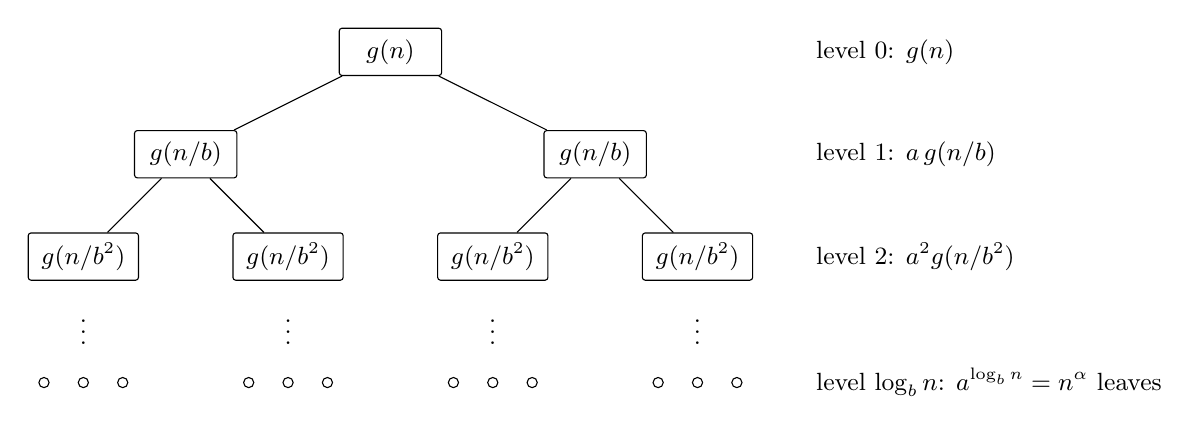
\begin{tikzpicture}[ads,
    rec/.style={draw,rounded corners=1pt,minimum height=6mm,
                minimum width=13mm,font=\small},
    lvl/.style={font=\small,anchor=west}]
  \node[rec] (r) at (0,0) {$g( n )$};
  \node[rec] (a) at (-2.6,-1.3) {$g( n / b )$};
  \node[rec] (b) at (2.6,-1.3) {$g( n / b )$};
  \foreach \k/\x in {1/-3.9,2/-1.3,3/1.3,4/3.9}
    \node[rec,minimum width=14mm] (l\k) at (\x,-2.6) {$g( n / b^2 )$};
  \draw (r) -- (a); \draw (r) -- (b);
  \draw (a) -- (l1); \draw (a) -- (l2);
  \draw (b) -- (l3); \draw (b) -- (l4);
  \foreach \x in {-3.9,-1.3,1.3,3.9}
    \node[font=\small] at (\x,-3.45) {$\vdots$};
  \foreach \x in {-4.4,-3.9,-3.4,-1.8,-1.3,-0.8,0.8,1.3,1.8,3.4,3.9,4.4}
    \node[draw,circle,inner sep=1.3pt] at (\x,-4.2) {};
  \node[lvl] at (5.4,0) {level 0: $g( n )$};
  \node[lvl] at (5.4,-1.3) {level 1: $a \, g( n / b )$};
  \node[lvl] at (5.4,-2.6) {level 2: $a^2 g( n / b^2 )$};
  \node[lvl] at (5.4,-4.2) {level $\log_b n$: $a^{\log_b n} = n^\alpha$ leaves};
\end{tikzpicture}
\end{document}
